\documentclass{article}
\usepackage{amsmath, sfmath, multicol, tkz-euclide, array, enumerate, tcolorbox, tabularray}
\renewcommand{\familydefault}{\sfdefault}
\setlength{\parindent}{0cm}
\pagestyle{empty}
\usepackage[left=1in, top=0.5in, right=1in, bottom=0.5in]{geometry}
\tikzset{>=stealth, label style/.append style={font=\footnotesize}}
\tcbset{colback=white}

\newcounter{example}[section]
\newenvironment{example}[1][]{\refstepcounter{example}\par\medskip
   {\color{red}\textbf{Example~\theexample. #1}}}{\medskip}

\begin{document}

\section*{Areas of Regular Polygons}

\begin{tcolorbox}[colframe=orange!70!white, coltitle=black, title=\textbf{Today I Can}]
\begin{enumerate}
    \item Determine the area of regular polygons.
\end{enumerate}
\end{tcolorbox}
\bigskip 

\begin{center}
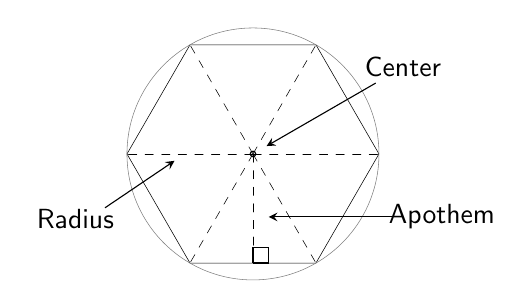
\begin{tikzpicture}[scale=0.8]
\tkzDefPoints{0/0/O, 2/0/A, -2/0/D}
\tkzDefShiftPoint[O](60:2){B}
\tkzDefShiftPoint[O](120:2){C}
\tkzDefShiftPoint[O](240:2){E}
\tkzDefShiftPoint[O](300:2){F}
\tkzDrawPolygon(A,B,C,D,E,F)
\tkzDrawPoint(O)
\tkzDefMidPoint(E,F)
\tkzGetPoint{G}
\tkzDrawSegments[dashed](O,A O,B O,C O,D O,E O,F O,G)
\tkzDrawCircle(O,A)
\node at (200:3) {Radius};
\draw [->, >=stealth] (200:2.5) -- (185:1.25);
\node at (3,-1) {Apothem};
\draw [->, >=stealth] (2.25,-1) -- (0.25,-1);
\node at (30:2.75) {Center};
\draw [->, >=stealth] (30:2.25) -- (30:0.25);
\tkzMarkRightAngle(F,G,O)
\end{tikzpicture}
\end{center}

\begin{tcolorbox}[colframe=black!20!white, opacitybacktitle=0.1, coltitle=black, title=\textbf{Area of Regular Polygon}]
\begin{minipage}{0.5\textwidth}
\begin{itemize}
    \item $\text{Area } = \frac{1}{2}aP$
\end{itemize}
\end{minipage}
\begin{minipage}{0.4\textwidth}
    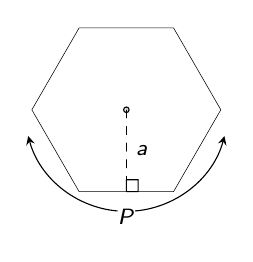
\begin{tikzpicture}[scale=0.6]
    \tkzDefPoints{0/0/O, 2/0/A, -2/0/D}
    \tkzDefShiftPoint[O](60:2){B}
    \tkzDefShiftPoint[O](120:2){C}
    \tkzDefShiftPoint[O](240:2){E}
    \tkzDefShiftPoint[O](300:2){F}
    \tkzDrawPolygon(A,B,C,D,E,F)
    \tkzDrawPoint(O)
    \tkzDefMidPoint(E,F)
    \tkzGetPoint{G}
    \tkzDrawSegments[dashed](O,G)
    \tkzLabelSegment[right](O,G){$a$}
    \tkzMarkRightAngle(F,G,O)
    \tkzLabelSegment[below, yshift=-0.1cm](E,F){$P$}
    \draw [->, >=stealth] (275:2.15) arc (275:345:2.15);
    \draw [->, >=stealth] (265:2.15) arc (265:195:2.15);
    \end{tikzpicture}
\end{minipage}
\end{tcolorbox}
\bigskip 

\begin{example}
What is the area of each?
\begin{multicols}{2}
\begin{enumerate}[(a)]
    \item \mbox{} \newline 
    \item \mbox{} \newline 
\end{enumerate}
\end{multicols}
\begin{minipage}{0.5\textwidth}
    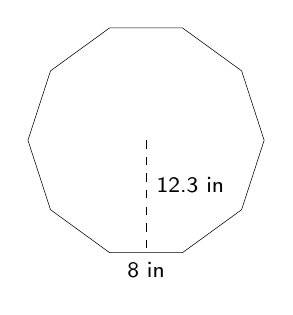
\begin{tikzpicture}[scale=0.75]
    \tkzDefPoints{0/0/O, 2/0/A, -2/0/F}
    \tkzDefShiftPoint[O](36:2){B}
    \tkzDefShiftPoint[O](72:2){C}
    \tkzDefShiftPoint[O](108:2){D}
    \tkzDefShiftPoint[O](144:2){E}
    \tkzDefShiftPoint[O](216:2){G}
    \tkzDefShiftPoint[O](252:2){H}
    \tkzDefShiftPoint[O](288:2){I}
    \tkzDefShiftPoint[O](324:2){J}
    \tkzDrawPolygon(A,B,C,D,E,F,G,H,I,J)
    \draw [dashed] (O) -- (270:1.95);
    \node at (0.75,-0.75) {\footnotesize 12.3 in};
    \tkzLabelSegment[below](H,I){\footnotesize 8 in}
    \end{tikzpicture}
\end{minipage}
\begin{minipage}{0.4\textwidth}
    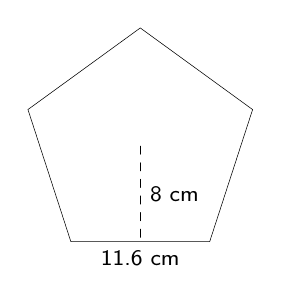
\begin{tikzpicture}[scale=0.75]
    \tkzDefPoints{0/0/O, 0/2/A}
    \tkzDefShiftPoint[O](162:2){B}
    \tkzDefShiftPoint[O](234:2){C}
    \tkzDefShiftPoint[O](306:2){D}
    \tkzDefShiftPoint[O](378:2){E}
    \tkzDrawPolygon(A,B,C,D,E)
    \tkzDefMidPoint(C,D)
    \tkzGetPoint{F}
    \tkzDrawSegment[dashed](O,F)
    \tkzLabelSegment[below](D,C){11.6 cm}
    \tkzLabelSegment[right](O,F){8 cm}
    \end{tikzpicture}
\end{minipage}
\end{example}

\vspace{0.25in}

\textsc{Finding the Height of an Equilateral Triangle}:
\begin{enumerate}
    \item Divide side by 2.
    \item Multiply that by $\sqrt{3}$.
\end{enumerate}
\bigskip 

\begin{example}
A honeycomb is made up of regular hexagonal cells. The length of a side of a cell is 3 mm. What is the area of the cell?
\end{example}

\vfill 

\begin{example}
The side of a regular hexagon is 16 ft. What is the exact area of the hexagon?
\end{example}

\vfill 
\end{document}
